\renewcommand{\theequation}{\theenumi}
\begin{enumerate}[label=\arabic*.,ref=\thesubsection.\theenumi]
\numberwithin{equation}{enumi}
\item  Equal chords of a circle (or of congruent circles) subtend equal angles at the centre. 
\item  If the angles subtended by two chords of a circle (or of congruent circles) at the centre (corresponding centres) are equal, the chords are equal.
\item  The perpendicular from the centre of a circle to a chord bisects the chord. 
\item  The line drawn through the centre of a circle to bisect a chord is perpendicular to the chord.
\item  There is one and only one circle passing through three non-collinear points. 
\item  Equal chords of a circle (or of congruent circles) are equidistant from the centre (or corresponding centres).
\item Chords equidistant from the centre (or corresponding centres) of a circle (or of congruent circles) are equal.
\item  If two arcs of a circle are congruent, then their corresponding chords are equal and conversely if two chords of a circle are equal, then their corresponding arcs (minor, major) are congruent.
\item Congruent arcs of a circle subtend equal angles at the centre. 
\item  The angle subtended by an arc at the centre is double the angle subtended by it at any point on the remaining part of the circle.
\item Angles in the same segment of a circle are equal. \item  Angle in a semicircle is a right angle. 
\item  If a line segment joining two points subtends equal angles at two other points lying on the same side of the line containing the line segment, the four points lie on a circle. 
\begin{enumerate}
\begin{figure}[!ht]
\centering
\resizebox{\columnwidth}{!}{%Exercise 8.1 prob 47
\begin{tikzpicture}
[scale=0.5,>=stealth,point/.style={draw,circle,fill = black,inner sep=0.5pt},]
%\tikzset{shift={(-3,0)}}
%Triangle sides
\def\a{4}
\def\c{9}
\def\xA{4}
\def\h{3}
\def\k{1}
%\def\c{7.5}
\def\yE{\h/2}
%Labeling points
\node (D) at (0,0)[point,label=below left:$D$] {};
\node (B) at ({\xA+\a}, \h )[point,label=above right:$B$] {};
\node (C) at (\c, 0)[point,label=below right:$C$] {};
%\node (E) at (2, \yE)
%\node (F) at (8.5, \yE)[point,label=below right:$F$] {};
%\node (M) at (\xA,\yE)[point,label=above right:$M$] {};
%\node (N) at ({\xA+\a}, \yE)[point,label=above left:$N$] {};
%\node (X) at (\xA , 0)[point,label=below left:$X$] {};
%\node (Y) at ({\xA+\a}, 0)[point,label=below right:$Y$] {};
\node (A) at (\xA , \h)[point,label=above left:$A$] {};
\node (E) at ($(D)!0.5!(A)$)[point,label=above left:$E$] {};
\node (F) at ($(B)!0.5!(C)$)[point,label=above right:$F$] {};



%A



%Drawing parallelogram ABCD
\draw (A) -- (B)--(C) --(D)--(A);
%\draw (A) --(X);
\draw (E) --(F);
\draw(A)--node[right]{$\textrm{k}$} (E)--node[right]{$\textrm{1}$} (D);
\draw(B)--node[left]{$\textrm{m}$} (F)--node[left]{$\textrm{1}$} (C);


%\draw (B) --(Y);
%marking right angles
%\tkzMarkRightAngle[fill=green!20,size=.2](D,X,A)
%\tkzMarkRightAngle[fill=green!20,size=.2](C,Y,B)


%
\end{tikzpicture}
}
\caption{}
\label{fig:8.1.47_trapezium_ABCD}	
\end{figure}

\item {\em Construction: }See Fig. \ref{fig:8.1.47_trapezium_ABCD}.
The input parameters are
\begin{align}
\label{eq:8.1.47_constr_d}
\vec{D} &= \myvec{0\\0} 
\\
\vec{C} &= \myvec{c\\0} 
\\
\vec{A} &= \myvec{p\\q} 
\\
\vec{B} &= \myvec{b\\q}, \quad b < c 
\label{eq:8.1.47_constr_c}
\end{align}
%
For $0 < k < 1$, 
\begin{align}
\label{eq:8.1.47_constr_e}
\vec{E} &= \frac{{k\vec{D} +\vec{A}}}{k+1}
\\
\vec{F} &= \frac{{k\vec{C} +\vec{B}}}{k+1}
\label{eq:8.1.47_constr_f}
\end{align}


The given curve 
\begin{align}
	y =\frac{1}{x-1}
\end{align}
can be expressed as 
\begin{align}
	xy - y - 1 = 0 \label{eq:solutions/1/14/eq:hyperbola}
\end{align}
Hence, we have
\begin{align}
	\vec{V} = \frac{1}{2}\myvec{0 & 1 \\ 1 & 0}, 
	\vec{u} = \frac{1}{2}\myvec{0 \\-1},
	f = -1
\end{align}
Since $\mydet{\vec{V}} < 0$, the equation \eqref{eq:solutions/1/14/eq:hyperbola} represents hyperbola.
To find the values of $\lambda_1$ and $\lambda_2$, consider the characteristic equation,
\begin{align}
	\mydet{\lambda\vec{I} - \vec{V}} &= 0\\
	\implies \mydet{\myvec{\lambda & 0\\0 & \lambda} - \myvec{0 & \frac{1}{2} \\ \frac{1}{2} & 0}} &= 0\\
	\implies \mydet{ \lambda & \frac{-1}{2} \\ \frac{-1}{2} & \lambda} &= 0\\
	\implies \lambda_1 &= \frac{1}{2} , \lambda_2 = \frac{-1}{2}
\end{align}
In addition, given the slope -1, the direction and normal vectors are given by 
\begin{align}
	\vec{m} = \myvec{1 \\ -1} \\
	\vec{n} = \myvec{ 1 \\ 1}
\end{align}
The parameters of hyperbola are as follows:
\begin{align}
	\vec{c} &= -\vec{V}^{-1}\vec{u} \\
	&= -\myvec{0 & 2\\ 2 & 0}\myvec{0 \\ -\frac{1}{2}} \\
	&= \myvec{1 \\ 0}\\
	axes &= \begin{cases}
	\sqrt{\frac{\vec{u}^T\vec{V}^{-1}\vec{u} - f}{\lambda_1}} = \sqrt{2}\\
 \sqrt{\frac{f-\vec{u}^T\vec{V}^{-1}\vec{u}}{\lambda_2}} = \sqrt{2}
\end{cases}
\end{align}
which represents the standard hyperbola equation,
\begin{align}
	\frac{x^2}{2} - \frac{x^2}{2} = 1
\end{align}
The points of contact are given by 
\begin{align}
  \tiny{K} &=\pm \sqrt{\frac{\vec{u}^T\vec{V}^{-1}\vec{u} - f}{\vec{n}^T\vec{V}^{-1}\vec{n}}}
  = \pm \frac{1}{2}\\
  \vec{q} &= \vec{V}^{-1}(k\vec{n}-\vec{u})\\
  \vec{q_1} &= \myvec{0 & 2\\2 & 0} \sbrak{\frac{1}{2}\myvec{1 \\ 1} - \myvec{0\\ \frac{-1}{2}}}\\
  &= \myvec{2 \\ 1}\\
  \vec{q_2} &= \myvec{0 & 2\\2 & 0} \sbrak{\frac{-1}{2}\myvec{1 \\ 1} - \myvec{0\\ \frac{-1}{2}}}\\
  &= \myvec{0 \\ -1}
\end{align} 
$\therefore$ The tangents are given by
\begin{align}
	\myvec{1 & 1} \brak{\vec{x} - \myvec{2 \\ 1}} = 0 \\
	\myvec{1 & 1} \brak{\vec{x} - \myvec{0 \\ -1}} = 0
\end{align}
The desired equations of all lines having slope -1 that are tangents to the curve $\frac{1}{x-1}, x \neq 1$ are given by
\begin{align}
	\myvec{1 & 1}\vec{x} &= 3 \\
	\myvec{1 & 1}\vec{x} &= -1 
\end{align}
The above results are verified in the following figure.
\begin{figure}[h!] \label{eq:solutions/1/14/fig:tangents}
	\centering
	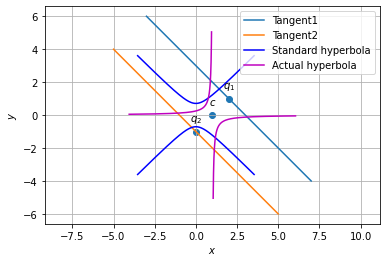
\includegraphics[width=\columnwidth]{./solutions/1/14/graph7.png}
	\caption{The standard and actual hyperbola.}
\end{figure}

\end{enumerate}
\item  The sum of either pair of opposite angles of a cyclic quadrilateral is 180$\degree$.
\item  If sum of a pair of opposite angles of a quadrilateral is 180$\degree$, the quadrilateral is cyclic.
%
\item AB is a diameter of the circle, $CD$ is a chord equal to the radius of the circle. $AC$ and $BD$ when extended intersect at a point $E$. Prove that $\angle AEB = 60\degree$.
\begin{enumerate}
\begin{figure}[!ht]
\centering
\resizebox{\columnwidth}{!}{%Exercise 8.1 prob 47
\begin{tikzpicture}
[scale=0.5,>=stealth,point/.style={draw,circle,fill = black,inner sep=0.5pt},]
%\tikzset{shift={(-3,0)}}
%Triangle sides
\def\a{4}
\def\c{9}
\def\xA{4}
\def\h{3}
\def\k{1}
%\def\c{7.5}
\def\yE{\h/2}
%Labeling points
\node (D) at (0,0)[point,label=below left:$D$] {};
\node (B) at ({\xA+\a}, \h )[point,label=above right:$B$] {};
\node (C) at (\c, 0)[point,label=below right:$C$] {};
%\node (E) at (2, \yE)
%\node (F) at (8.5, \yE)[point,label=below right:$F$] {};
%\node (M) at (\xA,\yE)[point,label=above right:$M$] {};
%\node (N) at ({\xA+\a}, \yE)[point,label=above left:$N$] {};
%\node (X) at (\xA , 0)[point,label=below left:$X$] {};
%\node (Y) at ({\xA+\a}, 0)[point,label=below right:$Y$] {};
\node (A) at (\xA , \h)[point,label=above left:$A$] {};
\node (E) at ($(D)!0.5!(A)$)[point,label=above left:$E$] {};
\node (F) at ($(B)!0.5!(C)$)[point,label=above right:$F$] {};



%A



%Drawing parallelogram ABCD
\draw (A) -- (B)--(C) --(D)--(A);
%\draw (A) --(X);
\draw (E) --(F);
\draw(A)--node[right]{$\textrm{k}$} (E)--node[right]{$\textrm{1}$} (D);
\draw(B)--node[left]{$\textrm{m}$} (F)--node[left]{$\textrm{1}$} (C);


%\draw (B) --(Y);
%marking right angles
%\tkzMarkRightAngle[fill=green!20,size=.2](D,X,A)
%\tkzMarkRightAngle[fill=green!20,size=.2](C,Y,B)


%
\end{tikzpicture}
}
\caption{}
\label{fig:8.1.47_trapezium_ABCD}	
\end{figure}

\item {\em Construction: }See Fig. \ref{fig:8.1.47_trapezium_ABCD}.
The input parameters are
\begin{align}
\label{eq:8.1.47_constr_d}
\vec{D} &= \myvec{0\\0} 
\\
\vec{C} &= \myvec{c\\0} 
\\
\vec{A} &= \myvec{p\\q} 
\\
\vec{B} &= \myvec{b\\q}, \quad b < c 
\label{eq:8.1.47_constr_c}
\end{align}
%
For $0 < k < 1$, 
\begin{align}
\label{eq:8.1.47_constr_e}
\vec{E} &= \frac{{k\vec{D} +\vec{A}}}{k+1}
\\
\vec{F} &= \frac{{k\vec{C} +\vec{B}}}{k+1}
\label{eq:8.1.47_constr_f}
\end{align}


The given curve 
\begin{align}
	y =\frac{1}{x-1}
\end{align}
can be expressed as 
\begin{align}
	xy - y - 1 = 0 \label{eq:solutions/1/14/eq:hyperbola}
\end{align}
Hence, we have
\begin{align}
	\vec{V} = \frac{1}{2}\myvec{0 & 1 \\ 1 & 0}, 
	\vec{u} = \frac{1}{2}\myvec{0 \\-1},
	f = -1
\end{align}
Since $\mydet{\vec{V}} < 0$, the equation \eqref{eq:solutions/1/14/eq:hyperbola} represents hyperbola.
To find the values of $\lambda_1$ and $\lambda_2$, consider the characteristic equation,
\begin{align}
	\mydet{\lambda\vec{I} - \vec{V}} &= 0\\
	\implies \mydet{\myvec{\lambda & 0\\0 & \lambda} - \myvec{0 & \frac{1}{2} \\ \frac{1}{2} & 0}} &= 0\\
	\implies \mydet{ \lambda & \frac{-1}{2} \\ \frac{-1}{2} & \lambda} &= 0\\
	\implies \lambda_1 &= \frac{1}{2} , \lambda_2 = \frac{-1}{2}
\end{align}
In addition, given the slope -1, the direction and normal vectors are given by 
\begin{align}
	\vec{m} = \myvec{1 \\ -1} \\
	\vec{n} = \myvec{ 1 \\ 1}
\end{align}
The parameters of hyperbola are as follows:
\begin{align}
	\vec{c} &= -\vec{V}^{-1}\vec{u} \\
	&= -\myvec{0 & 2\\ 2 & 0}\myvec{0 \\ -\frac{1}{2}} \\
	&= \myvec{1 \\ 0}\\
	axes &= \begin{cases}
	\sqrt{\frac{\vec{u}^T\vec{V}^{-1}\vec{u} - f}{\lambda_1}} = \sqrt{2}\\
 \sqrt{\frac{f-\vec{u}^T\vec{V}^{-1}\vec{u}}{\lambda_2}} = \sqrt{2}
\end{cases}
\end{align}
which represents the standard hyperbola equation,
\begin{align}
	\frac{x^2}{2} - \frac{x^2}{2} = 1
\end{align}
The points of contact are given by 
\begin{align}
  \tiny{K} &=\pm \sqrt{\frac{\vec{u}^T\vec{V}^{-1}\vec{u} - f}{\vec{n}^T\vec{V}^{-1}\vec{n}}}
  = \pm \frac{1}{2}\\
  \vec{q} &= \vec{V}^{-1}(k\vec{n}-\vec{u})\\
  \vec{q_1} &= \myvec{0 & 2\\2 & 0} \sbrak{\frac{1}{2}\myvec{1 \\ 1} - \myvec{0\\ \frac{-1}{2}}}\\
  &= \myvec{2 \\ 1}\\
  \vec{q_2} &= \myvec{0 & 2\\2 & 0} \sbrak{\frac{-1}{2}\myvec{1 \\ 1} - \myvec{0\\ \frac{-1}{2}}}\\
  &= \myvec{0 \\ -1}
\end{align} 
$\therefore$ The tangents are given by
\begin{align}
	\myvec{1 & 1} \brak{\vec{x} - \myvec{2 \\ 1}} = 0 \\
	\myvec{1 & 1} \brak{\vec{x} - \myvec{0 \\ -1}} = 0
\end{align}
The desired equations of all lines having slope -1 that are tangents to the curve $\frac{1}{x-1}, x \neq 1$ are given by
\begin{align}
	\myvec{1 & 1}\vec{x} &= 3 \\
	\myvec{1 & 1}\vec{x} &= -1 
\end{align}
The above results are verified in the following figure.
\begin{figure}[h!] \label{eq:solutions/1/14/fig:tangents}
	\centering
	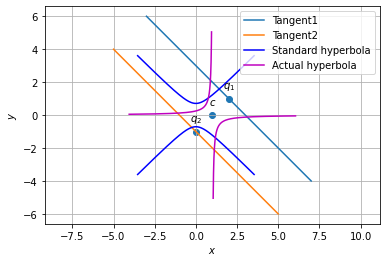
\includegraphics[width=\columnwidth]{./solutions/1/14/graph7.png}
	\caption{The standard and actual hyperbola.}
\end{figure}

\end{enumerate}

\item $ABCD$ is a cyclic quadrilateral in which $AC$ and $BD$ are its diagonals. If $\angle DBC = 55\degree$ and $\angle BAC = 45\degree$, find $\angle BCD$
\item Two circles intersect at two points $A and B$. $AD$ and $AC$ are diameters to the two circles. Prove that $B$ lies on the line segment $DC$.
\item Prove that the quadrilateral formed (if possible) by the internal angle bisectors of any quadrilateral is cyclic.
\begin{enumerate}
\begin{figure}[!ht]
\centering
\resizebox{\columnwidth}{!}{%Exercise 8.1 prob 47
\begin{tikzpicture}
[scale=0.5,>=stealth,point/.style={draw,circle,fill = black,inner sep=0.5pt},]
%\tikzset{shift={(-3,0)}}
%Triangle sides
\def\a{4}
\def\c{9}
\def\xA{4}
\def\h{3}
\def\k{1}
%\def\c{7.5}
\def\yE{\h/2}
%Labeling points
\node (D) at (0,0)[point,label=below left:$D$] {};
\node (B) at ({\xA+\a}, \h )[point,label=above right:$B$] {};
\node (C) at (\c, 0)[point,label=below right:$C$] {};
%\node (E) at (2, \yE)
%\node (F) at (8.5, \yE)[point,label=below right:$F$] {};
%\node (M) at (\xA,\yE)[point,label=above right:$M$] {};
%\node (N) at ({\xA+\a}, \yE)[point,label=above left:$N$] {};
%\node (X) at (\xA , 0)[point,label=below left:$X$] {};
%\node (Y) at ({\xA+\a}, 0)[point,label=below right:$Y$] {};
\node (A) at (\xA , \h)[point,label=above left:$A$] {};
\node (E) at ($(D)!0.5!(A)$)[point,label=above left:$E$] {};
\node (F) at ($(B)!0.5!(C)$)[point,label=above right:$F$] {};



%A



%Drawing parallelogram ABCD
\draw (A) -- (B)--(C) --(D)--(A);
%\draw (A) --(X);
\draw (E) --(F);
\draw(A)--node[right]{$\textrm{k}$} (E)--node[right]{$\textrm{1}$} (D);
\draw(B)--node[left]{$\textrm{m}$} (F)--node[left]{$\textrm{1}$} (C);


%\draw (B) --(Y);
%marking right angles
%\tkzMarkRightAngle[fill=green!20,size=.2](D,X,A)
%\tkzMarkRightAngle[fill=green!20,size=.2](C,Y,B)


%
\end{tikzpicture}
}
\caption{}
\label{fig:8.1.47_trapezium_ABCD}	
\end{figure}

\item {\em Construction: }See Fig. \ref{fig:8.1.47_trapezium_ABCD}.
The input parameters are
\begin{align}
\label{eq:8.1.47_constr_d}
\vec{D} &= \myvec{0\\0} 
\\
\vec{C} &= \myvec{c\\0} 
\\
\vec{A} &= \myvec{p\\q} 
\\
\vec{B} &= \myvec{b\\q}, \quad b < c 
\label{eq:8.1.47_constr_c}
\end{align}
%
For $0 < k < 1$, 
\begin{align}
\label{eq:8.1.47_constr_e}
\vec{E} &= \frac{{k\vec{D} +\vec{A}}}{k+1}
\\
\vec{F} &= \frac{{k\vec{C} +\vec{B}}}{k+1}
\label{eq:8.1.47_constr_f}
\end{align}


The given curve 
\begin{align}
	y =\frac{1}{x-1}
\end{align}
can be expressed as 
\begin{align}
	xy - y - 1 = 0 \label{eq:solutions/1/14/eq:hyperbola}
\end{align}
Hence, we have
\begin{align}
	\vec{V} = \frac{1}{2}\myvec{0 & 1 \\ 1 & 0}, 
	\vec{u} = \frac{1}{2}\myvec{0 \\-1},
	f = -1
\end{align}
Since $\mydet{\vec{V}} < 0$, the equation \eqref{eq:solutions/1/14/eq:hyperbola} represents hyperbola.
To find the values of $\lambda_1$ and $\lambda_2$, consider the characteristic equation,
\begin{align}
	\mydet{\lambda\vec{I} - \vec{V}} &= 0\\
	\implies \mydet{\myvec{\lambda & 0\\0 & \lambda} - \myvec{0 & \frac{1}{2} \\ \frac{1}{2} & 0}} &= 0\\
	\implies \mydet{ \lambda & \frac{-1}{2} \\ \frac{-1}{2} & \lambda} &= 0\\
	\implies \lambda_1 &= \frac{1}{2} , \lambda_2 = \frac{-1}{2}
\end{align}
In addition, given the slope -1, the direction and normal vectors are given by 
\begin{align}
	\vec{m} = \myvec{1 \\ -1} \\
	\vec{n} = \myvec{ 1 \\ 1}
\end{align}
The parameters of hyperbola are as follows:
\begin{align}
	\vec{c} &= -\vec{V}^{-1}\vec{u} \\
	&= -\myvec{0 & 2\\ 2 & 0}\myvec{0 \\ -\frac{1}{2}} \\
	&= \myvec{1 \\ 0}\\
	axes &= \begin{cases}
	\sqrt{\frac{\vec{u}^T\vec{V}^{-1}\vec{u} - f}{\lambda_1}} = \sqrt{2}\\
 \sqrt{\frac{f-\vec{u}^T\vec{V}^{-1}\vec{u}}{\lambda_2}} = \sqrt{2}
\end{cases}
\end{align}
which represents the standard hyperbola equation,
\begin{align}
	\frac{x^2}{2} - \frac{x^2}{2} = 1
\end{align}
The points of contact are given by 
\begin{align}
  \tiny{K} &=\pm \sqrt{\frac{\vec{u}^T\vec{V}^{-1}\vec{u} - f}{\vec{n}^T\vec{V}^{-1}\vec{n}}}
  = \pm \frac{1}{2}\\
  \vec{q} &= \vec{V}^{-1}(k\vec{n}-\vec{u})\\
  \vec{q_1} &= \myvec{0 & 2\\2 & 0} \sbrak{\frac{1}{2}\myvec{1 \\ 1} - \myvec{0\\ \frac{-1}{2}}}\\
  &= \myvec{2 \\ 1}\\
  \vec{q_2} &= \myvec{0 & 2\\2 & 0} \sbrak{\frac{-1}{2}\myvec{1 \\ 1} - \myvec{0\\ \frac{-1}{2}}}\\
  &= \myvec{0 \\ -1}
\end{align} 
$\therefore$ The tangents are given by
\begin{align}
	\myvec{1 & 1} \brak{\vec{x} - \myvec{2 \\ 1}} = 0 \\
	\myvec{1 & 1} \brak{\vec{x} - \myvec{0 \\ -1}} = 0
\end{align}
The desired equations of all lines having slope -1 that are tangents to the curve $\frac{1}{x-1}, x \neq 1$ are given by
\begin{align}
	\myvec{1 & 1}\vec{x} &= 3 \\
	\myvec{1 & 1}\vec{x} &= -1 
\end{align}
The above results are verified in the following figure.
\begin{figure}[h!] \label{eq:solutions/1/14/fig:tangents}
	\centering
	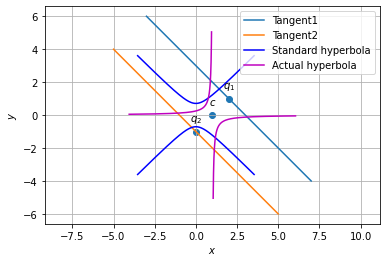
\includegraphics[width=\columnwidth]{./solutions/1/14/graph7.png}
	\caption{The standard and actual hyperbola.}
\end{figure}

\end{enumerate}

\item  Equal chords of a circle (or of congruent circles) subtend equal angles at the centre. 
\item  If the angles subtended by two chords of a circle (or of congruent circles) at the centre (corresponding centres) are equal, the chords are equal.
\item  The perpendicular from the centre of a circle to a chord bisects the chord. 
\item  The line drawn through the centre of a circle to bisect a chord is perpendicular to the chord.
\item  There is one and only one circle passing through three non-collinear points. 
\item  Equal chords of a circle (or of congruent circles) are equidistant from the centre (or corresponding centres).
\item Chords equidistant from the centre (or corresponding centres) of a circle (or of congruent circles) are equal.
\item  If two arcs of a circle are congruent, then their corresponding chords are equal and conversely if two chords of a circle are equal, then their corresponding arcs (minor, major) are congruent.
\item Congruent arcs of a circle subtend equal angles at the centre. 
\item  The angle subtended by an arc at the centre is double the angle subtended by it at any point on the remaining part of the circle.
\item Angles in the same segment of a circle are equal. \item  Angle in a semicircle is a right angle. 
\item  If a line segment joining two points subtends equal angles at two other points lying on the same side of the line containing the line segment, the four points lie on a circle. 
\item  The sum of either pair of opposite angles of a cyclic quadrilateral is 180$\degree$.
\item  If sum of a pair of opposite angles of a quadrilateral is 180$\degree$, the quadrilateral is cyclic.
%
\item AB is a diameter of the circle, $CD$ is a chord equal to the radius of the circle. $AC$ and $BD$ when extended intersect at a point $E$. Prove that $\angle AEB = 60\degree$.
\item Two circles intersect at two points $A$ and $B$. $AD$ and $AC$ are diameters to the two circles. Prove that $B$ lies on the line segment $DC$.
\item Prove that the quadrilateral formed (if possible) by the internal angle bisectors of any quadrilateral is cyclic.
\item  If two equal chords of a circle intersect within the circle, prove that the segments of one chord are equal to corresponding segments of the other chord.
\item If two equal chords of a circle intersect within the circle, prove that the line joining the point of intersection to the centre makes equal angles with the chords.
\begin{enumerate}
\begin{figure}[!ht]
\centering
\resizebox{\columnwidth}{!}{%Exercise 8.1 prob 47
\begin{tikzpicture}
[scale=0.5,>=stealth,point/.style={draw,circle,fill = black,inner sep=0.5pt},]
%\tikzset{shift={(-3,0)}}
%Triangle sides
\def\a{4}
\def\c{9}
\def\xA{4}
\def\h{3}
\def\k{1}
%\def\c{7.5}
\def\yE{\h/2}
%Labeling points
\node (D) at (0,0)[point,label=below left:$D$] {};
\node (B) at ({\xA+\a}, \h )[point,label=above right:$B$] {};
\node (C) at (\c, 0)[point,label=below right:$C$] {};
%\node (E) at (2, \yE)
%\node (F) at (8.5, \yE)[point,label=below right:$F$] {};
%\node (M) at (\xA,\yE)[point,label=above right:$M$] {};
%\node (N) at ({\xA+\a}, \yE)[point,label=above left:$N$] {};
%\node (X) at (\xA , 0)[point,label=below left:$X$] {};
%\node (Y) at ({\xA+\a}, 0)[point,label=below right:$Y$] {};
\node (A) at (\xA , \h)[point,label=above left:$A$] {};
\node (E) at ($(D)!0.5!(A)$)[point,label=above left:$E$] {};
\node (F) at ($(B)!0.5!(C)$)[point,label=above right:$F$] {};



%A



%Drawing parallelogram ABCD
\draw (A) -- (B)--(C) --(D)--(A);
%\draw (A) --(X);
\draw (E) --(F);
\draw(A)--node[right]{$\textrm{k}$} (E)--node[right]{$\textrm{1}$} (D);
\draw(B)--node[left]{$\textrm{m}$} (F)--node[left]{$\textrm{1}$} (C);


%\draw (B) --(Y);
%marking right angles
%\tkzMarkRightAngle[fill=green!20,size=.2](D,X,A)
%\tkzMarkRightAngle[fill=green!20,size=.2](C,Y,B)


%
\end{tikzpicture}
}
\caption{}
\label{fig:8.1.47_trapezium_ABCD}	
\end{figure}

\item {\em Construction: }See Fig. \ref{fig:8.1.47_trapezium_ABCD}.
The input parameters are
\begin{align}
\label{eq:8.1.47_constr_d}
\vec{D} &= \myvec{0\\0} 
\\
\vec{C} &= \myvec{c\\0} 
\\
\vec{A} &= \myvec{p\\q} 
\\
\vec{B} &= \myvec{b\\q}, \quad b < c 
\label{eq:8.1.47_constr_c}
\end{align}
%
For $0 < k < 1$, 
\begin{align}
\label{eq:8.1.47_constr_e}
\vec{E} &= \frac{{k\vec{D} +\vec{A}}}{k+1}
\\
\vec{F} &= \frac{{k\vec{C} +\vec{B}}}{k+1}
\label{eq:8.1.47_constr_f}
\end{align}


The given curve 
\begin{align}
	y =\frac{1}{x-1}
\end{align}
can be expressed as 
\begin{align}
	xy - y - 1 = 0 \label{eq:solutions/1/14/eq:hyperbola}
\end{align}
Hence, we have
\begin{align}
	\vec{V} = \frac{1}{2}\myvec{0 & 1 \\ 1 & 0}, 
	\vec{u} = \frac{1}{2}\myvec{0 \\-1},
	f = -1
\end{align}
Since $\mydet{\vec{V}} < 0$, the equation \eqref{eq:solutions/1/14/eq:hyperbola} represents hyperbola.
To find the values of $\lambda_1$ and $\lambda_2$, consider the characteristic equation,
\begin{align}
	\mydet{\lambda\vec{I} - \vec{V}} &= 0\\
	\implies \mydet{\myvec{\lambda & 0\\0 & \lambda} - \myvec{0 & \frac{1}{2} \\ \frac{1}{2} & 0}} &= 0\\
	\implies \mydet{ \lambda & \frac{-1}{2} \\ \frac{-1}{2} & \lambda} &= 0\\
	\implies \lambda_1 &= \frac{1}{2} , \lambda_2 = \frac{-1}{2}
\end{align}
In addition, given the slope -1, the direction and normal vectors are given by 
\begin{align}
	\vec{m} = \myvec{1 \\ -1} \\
	\vec{n} = \myvec{ 1 \\ 1}
\end{align}
The parameters of hyperbola are as follows:
\begin{align}
	\vec{c} &= -\vec{V}^{-1}\vec{u} \\
	&= -\myvec{0 & 2\\ 2 & 0}\myvec{0 \\ -\frac{1}{2}} \\
	&= \myvec{1 \\ 0}\\
	axes &= \begin{cases}
	\sqrt{\frac{\vec{u}^T\vec{V}^{-1}\vec{u} - f}{\lambda_1}} = \sqrt{2}\\
 \sqrt{\frac{f-\vec{u}^T\vec{V}^{-1}\vec{u}}{\lambda_2}} = \sqrt{2}
\end{cases}
\end{align}
which represents the standard hyperbola equation,
\begin{align}
	\frac{x^2}{2} - \frac{x^2}{2} = 1
\end{align}
The points of contact are given by 
\begin{align}
  \tiny{K} &=\pm \sqrt{\frac{\vec{u}^T\vec{V}^{-1}\vec{u} - f}{\vec{n}^T\vec{V}^{-1}\vec{n}}}
  = \pm \frac{1}{2}\\
  \vec{q} &= \vec{V}^{-1}(k\vec{n}-\vec{u})\\
  \vec{q_1} &= \myvec{0 & 2\\2 & 0} \sbrak{\frac{1}{2}\myvec{1 \\ 1} - \myvec{0\\ \frac{-1}{2}}}\\
  &= \myvec{2 \\ 1}\\
  \vec{q_2} &= \myvec{0 & 2\\2 & 0} \sbrak{\frac{-1}{2}\myvec{1 \\ 1} - \myvec{0\\ \frac{-1}{2}}}\\
  &= \myvec{0 \\ -1}
\end{align} 
$\therefore$ The tangents are given by
\begin{align}
	\myvec{1 & 1} \brak{\vec{x} - \myvec{2 \\ 1}} = 0 \\
	\myvec{1 & 1} \brak{\vec{x} - \myvec{0 \\ -1}} = 0
\end{align}
The desired equations of all lines having slope -1 that are tangents to the curve $\frac{1}{x-1}, x \neq 1$ are given by
\begin{align}
	\myvec{1 & 1}\vec{x} &= 3 \\
	\myvec{1 & 1}\vec{x} &= -1 
\end{align}
The above results are verified in the following figure.
\begin{figure}[h!] \label{eq:solutions/1/14/fig:tangents}
	\centering
	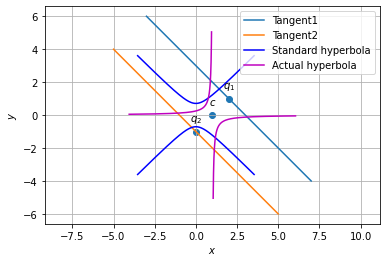
\includegraphics[width=\columnwidth]{./solutions/1/14/graph7.png}
	\caption{The standard and actual hyperbola.}
\end{figure}

\end{enumerate}

\item If a line intersects two concentric circles (circles with the same centre) with centre O at A, B, C and D, prove that AB = CD.
\begin{enumerate}
\begin{figure}[!ht]
\centering
\resizebox{\columnwidth}{!}{%Exercise 8.1 prob 47
\begin{tikzpicture}
[scale=0.5,>=stealth,point/.style={draw,circle,fill = black,inner sep=0.5pt},]
%\tikzset{shift={(-3,0)}}
%Triangle sides
\def\a{4}
\def\c{9}
\def\xA{4}
\def\h{3}
\def\k{1}
%\def\c{7.5}
\def\yE{\h/2}
%Labeling points
\node (D) at (0,0)[point,label=below left:$D$] {};
\node (B) at ({\xA+\a}, \h )[point,label=above right:$B$] {};
\node (C) at (\c, 0)[point,label=below right:$C$] {};
%\node (E) at (2, \yE)
%\node (F) at (8.5, \yE)[point,label=below right:$F$] {};
%\node (M) at (\xA,\yE)[point,label=above right:$M$] {};
%\node (N) at ({\xA+\a}, \yE)[point,label=above left:$N$] {};
%\node (X) at (\xA , 0)[point,label=below left:$X$] {};
%\node (Y) at ({\xA+\a}, 0)[point,label=below right:$Y$] {};
\node (A) at (\xA , \h)[point,label=above left:$A$] {};
\node (E) at ($(D)!0.5!(A)$)[point,label=above left:$E$] {};
\node (F) at ($(B)!0.5!(C)$)[point,label=above right:$F$] {};



%A



%Drawing parallelogram ABCD
\draw (A) -- (B)--(C) --(D)--(A);
%\draw (A) --(X);
\draw (E) --(F);
\draw(A)--node[right]{$\textrm{k}$} (E)--node[right]{$\textrm{1}$} (D);
\draw(B)--node[left]{$\textrm{m}$} (F)--node[left]{$\textrm{1}$} (C);


%\draw (B) --(Y);
%marking right angles
%\tkzMarkRightAngle[fill=green!20,size=.2](D,X,A)
%\tkzMarkRightAngle[fill=green!20,size=.2](C,Y,B)


%
\end{tikzpicture}
}
\caption{}
\label{fig:8.1.47_trapezium_ABCD}	
\end{figure}

\item {\em Construction: }See Fig. \ref{fig:8.1.47_trapezium_ABCD}.
The input parameters are
\begin{align}
\label{eq:8.1.47_constr_d}
\vec{D} &= \myvec{0\\0} 
\\
\vec{C} &= \myvec{c\\0} 
\\
\vec{A} &= \myvec{p\\q} 
\\
\vec{B} &= \myvec{b\\q}, \quad b < c 
\label{eq:8.1.47_constr_c}
\end{align}
%
For $0 < k < 1$, 
\begin{align}
\label{eq:8.1.47_constr_e}
\vec{E} &= \frac{{k\vec{D} +\vec{A}}}{k+1}
\\
\vec{F} &= \frac{{k\vec{C} +\vec{B}}}{k+1}
\label{eq:8.1.47_constr_f}
\end{align}


The given curve 
\begin{align}
	y =\frac{1}{x-1}
\end{align}
can be expressed as 
\begin{align}
	xy - y - 1 = 0 \label{eq:solutions/1/14/eq:hyperbola}
\end{align}
Hence, we have
\begin{align}
	\vec{V} = \frac{1}{2}\myvec{0 & 1 \\ 1 & 0}, 
	\vec{u} = \frac{1}{2}\myvec{0 \\-1},
	f = -1
\end{align}
Since $\mydet{\vec{V}} < 0$, the equation \eqref{eq:solutions/1/14/eq:hyperbola} represents hyperbola.
To find the values of $\lambda_1$ and $\lambda_2$, consider the characteristic equation,
\begin{align}
	\mydet{\lambda\vec{I} - \vec{V}} &= 0\\
	\implies \mydet{\myvec{\lambda & 0\\0 & \lambda} - \myvec{0 & \frac{1}{2} \\ \frac{1}{2} & 0}} &= 0\\
	\implies \mydet{ \lambda & \frac{-1}{2} \\ \frac{-1}{2} & \lambda} &= 0\\
	\implies \lambda_1 &= \frac{1}{2} , \lambda_2 = \frac{-1}{2}
\end{align}
In addition, given the slope -1, the direction and normal vectors are given by 
\begin{align}
	\vec{m} = \myvec{1 \\ -1} \\
	\vec{n} = \myvec{ 1 \\ 1}
\end{align}
The parameters of hyperbola are as follows:
\begin{align}
	\vec{c} &= -\vec{V}^{-1}\vec{u} \\
	&= -\myvec{0 & 2\\ 2 & 0}\myvec{0 \\ -\frac{1}{2}} \\
	&= \myvec{1 \\ 0}\\
	axes &= \begin{cases}
	\sqrt{\frac{\vec{u}^T\vec{V}^{-1}\vec{u} - f}{\lambda_1}} = \sqrt{2}\\
 \sqrt{\frac{f-\vec{u}^T\vec{V}^{-1}\vec{u}}{\lambda_2}} = \sqrt{2}
\end{cases}
\end{align}
which represents the standard hyperbola equation,
\begin{align}
	\frac{x^2}{2} - \frac{x^2}{2} = 1
\end{align}
The points of contact are given by 
\begin{align}
  \tiny{K} &=\pm \sqrt{\frac{\vec{u}^T\vec{V}^{-1}\vec{u} - f}{\vec{n}^T\vec{V}^{-1}\vec{n}}}
  = \pm \frac{1}{2}\\
  \vec{q} &= \vec{V}^{-1}(k\vec{n}-\vec{u})\\
  \vec{q_1} &= \myvec{0 & 2\\2 & 0} \sbrak{\frac{1}{2}\myvec{1 \\ 1} - \myvec{0\\ \frac{-1}{2}}}\\
  &= \myvec{2 \\ 1}\\
  \vec{q_2} &= \myvec{0 & 2\\2 & 0} \sbrak{\frac{-1}{2}\myvec{1 \\ 1} - \myvec{0\\ \frac{-1}{2}}}\\
  &= \myvec{0 \\ -1}
\end{align} 
$\therefore$ The tangents are given by
\begin{align}
	\myvec{1 & 1} \brak{\vec{x} - \myvec{2 \\ 1}} = 0 \\
	\myvec{1 & 1} \brak{\vec{x} - \myvec{0 \\ -1}} = 0
\end{align}
The desired equations of all lines having slope -1 that are tangents to the curve $\frac{1}{x-1}, x \neq 1$ are given by
\begin{align}
	\myvec{1 & 1}\vec{x} &= 3 \\
	\myvec{1 & 1}\vec{x} &= -1 
\end{align}
The above results are verified in the following figure.
\begin{figure}[h!] \label{eq:solutions/1/14/fig:tangents}
	\centering
	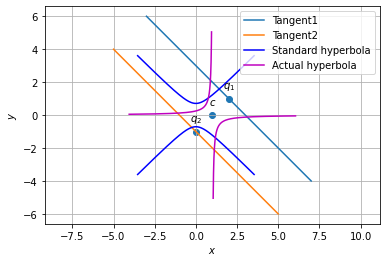
\includegraphics[width=\columnwidth]{./solutions/1/14/graph7.png}
	\caption{The standard and actual hyperbola.}
\end{figure}

\end{enumerate}
\item A chord of a circle is equal to the radius of the
circle. Find the angle subtended by the chord at
a point on the minor arc and also at a point on the
major arc.
\item If diagonals of a cyclic quadrilateral are diameters of the circle through the vertices of
the quadrilateral, prove that it is a rectangle.
\item If the non-parallel sides of a trapezium are equal, prove that it is cyclic.
\begin{enumerate}
\begin{figure}[!ht]
\centering
\resizebox{\columnwidth}{!}{\renewcommand{\theequation}{\theenumi}
\begin{enumerate}[label=\thesubsection.\arabic*.,ref=\thesubsection.\theenumi]
\numberwithin{equation}{enumi}
	%
%
\item 
%
Draw a circle of radius 3 units.Take two points P and Q on one its extended diameter each at a distance of 7 units from its centre. Draw tangents to the circle from these two points P and Q. 
\\
\solution The given parameters are listed in Table \ref{tab:table1}
%
\begin{table}[!ht]
\begin{center}
\begin{tabular}{ | m{2cm} | m{2cm} |} 
\hline
 & Circle \\
\hline
Centre  & $\vec{O}$=\myvec{0\\0} \\ 
\hline
Radius & $r$=3  \\ 
\hline
Radius & $d$=7  \\ 
\hline
\end{tabular}
\end{center}
\caption{Input values}
\label{tab:table1}
\end{table}
%
\begin{lemma}
  \label{lemma/linman/circ/contact/final}
  The points of contact for the tangent drawn from a point 
%
\begin{align}
  \vec{P} = d\vec{e}_1, \text{ where } \vec{e}_1 = \myvec{1\\0}
  \end{align}
  %
  to the circle are given by 
  \begin{align}
    \vec{x} = \frac{r^2}{d}\vec{e}_1  \pm r\sqrt{1 - \frac{r^2}{d^2}} \vec{e}_2
    \label{linman/circ/contact/final}
   \end{align}
%   
\end{lemma}
If $\vec{x}$ be a point of contact for the tangent from $\vec{P}$, 
\begin{align}
PR &\perp RO
\\
 \implies (\vec{O}-\vec{x})^{\top} (\vec{x}-\vec{P}) &= 0
 \\
 \text{or, }  \vec{P}^{\top} \vec{x} &=\norm{\vec{x}}^2 = r^2
 \\
 \implies \vec{e}_1^{\top} \vec{x} &= \frac{r^2}{d}
  \end{align}
  $\because \vec{O} = 0$.  The above equation can be expressed in parametric form as 
 \begin{align}
  \vec{x} = \frac{r^2}{d}\vec{e}_1 + \lambda \vec{e}_2
  \label{linman/circ/contact}
 \end{align}
 Substituting the above in 
 \begin{align}
  \norm{\vec{x}}^2 = r^2,
 \end{align}
 yields
\begin{align}
\norm{\frac{r^2}{d}\vec{e}_1 + \lambda \vec{e}_2}^2&=r^2
\\
\implies \lambda^2 &= r^2\sbrak{1 - \frac{r^2}{d^2}}
\\
\text{or, }\lambda &= \pm r\sqrt{1 - \frac{r^2}{d^2}}
\end{align}
%
Substituting $\lambda $ in \eqref{linman/circ/contact} yields \eqref{linman/circ/contact/final}.  Fig.  \ref{fig:Tangent lines to circle of radius 3 units.} shows all possible tangents
and their points of contact after substituting the numerical values in \eqref{linman/circ/contact/final}.
%
\begin{figure}[ht]
  \centering
  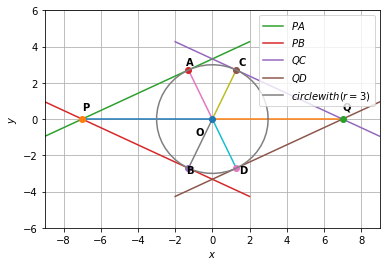
\includegraphics[width=\columnwidth]{solutions/su2021/circle/2/57/FIGURE3.png}
  \caption{Tangent lines to circle of radius 3 units.}
  \label{fig:Tangent lines to circle of radius 3 units.}
\end{figure}
%
\item Draw a  pair of tangents to a circle of radius 5 units  which are inclined to each other at an angle of $60\degree$.
\\
\solution  The angle between the tangents from $\vec{P}$ is given by 
\begin{lemma}
  Given a circle of radius $r$ and angle $\theta$ between the tangents, the intersection of the tangents and points of contact are
  given by Lemma   \ref{lemma/linman/circ/contact/final}  where 
  \begin{align}
    \implies d &= r\sin \frac{\theta}{2}
  \end{align}
%  
\end{lemma}
\begin{proof}
  From Fig.  \ref{fig:Tangent lines to circle of radius 3 units.},
\begin{align}
  \sin \frac{\theta}{2} &= \frac{r}{d}
  \\
  \implies d &= r\sin \frac{\theta}{2}
\end{align}
\end{proof}
Substituting numerical values and plotting, we obtain Fig. \ref{fig:Tangent lines to circle of radius 5 units.}.
%
\begin{figure}[ht]
  \centering
  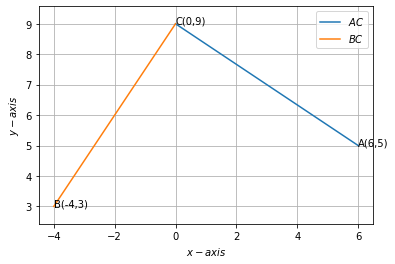
\includegraphics[width=\columnwidth]{solutions/su2021/circle/2/58/download.png}
  \caption{Tangent lines to circle of radius 5 units.}
  \label{fig:Tangent lines to circle of radius 5 units.}
\end{figure}   

\end{enumerate}
}
\caption{}
\label{fig:8.5.49_circle}	
\end{figure}
%
\item {\em Construction: }See Fig. \ref{fig:8.5.49_circle}.  The input parameters are
%
\begin{align}
\label{eq:8.5.49_constr_o}
\vec{O} &= \myvec{0\\0} 
\\
\vec{C} &= \myvec{r\\0} 
\label{eq:8.5.49_constr_c}
\end{align}
Then, 
%
\begin{align}
\label{eq:8.5.49_constr_a}
\vec{A} &= r\myvec{\cos \beta \\ -\sin \beta} 
\end{align}

\subitem Equal chords subtend equal angles at the centre.  Hence 
\begin{align}
\phase{EOC} &= \phase{AOD} = \frac{360 \degree - \alpha -\beta}{2}
\\
&= 180\degree - \frac{\alpha+\beta}{2}
\end{align}
Thus, 
\begin{align}
\vec{D} &= r\myvec{\cos \brak{180^{\circ}-\frac{\alpha+\beta}{2}+\alpha} \\ \sin \brak{180^{\circ}-\frac{\alpha+\beta}{2}+\alpha}} 
\\
 &= r\myvec{-\cos \frac{\alpha-\beta}{2} \\ -\sin \frac{\alpha-\beta}{2}}
\label{eq:8.5.49_constr_d}
\\
\vec{E} &= r\myvec{\cos \brak{180^{\circ}-\frac{\alpha+\beta}{2}} \\ \sin \brak{180^{\circ}-\frac{\alpha+\beta}{2}}}
\\
 &= r\myvec{-\cos \frac{\alpha+\beta}{2} \\ \sin \frac{\alpha+\beta}{2}}
\label{eq:8.5.49_constr_e}
\end{align}
\subitem $\vec{B}$ can be found as the intersection of $AD$ and $CE$.

The given curve 
\begin{align}
	y =\frac{1}{x-1}
\end{align}
can be expressed as 
\begin{align}
	xy - y - 1 = 0 \label{eq:solutions/1/14/eq:hyperbola}
\end{align}
Hence, we have
\begin{align}
	\vec{V} = \frac{1}{2}\myvec{0 & 1 \\ 1 & 0}, 
	\vec{u} = \frac{1}{2}\myvec{0 \\-1},
	f = -1
\end{align}
Since $\mydet{\vec{V}} < 0$, the equation \eqref{eq:solutions/1/14/eq:hyperbola} represents hyperbola.
To find the values of $\lambda_1$ and $\lambda_2$, consider the characteristic equation,
\begin{align}
	\mydet{\lambda\vec{I} - \vec{V}} &= 0\\
	\implies \mydet{\myvec{\lambda & 0\\0 & \lambda} - \myvec{0 & \frac{1}{2} \\ \frac{1}{2} & 0}} &= 0\\
	\implies \mydet{ \lambda & \frac{-1}{2} \\ \frac{-1}{2} & \lambda} &= 0\\
	\implies \lambda_1 &= \frac{1}{2} , \lambda_2 = \frac{-1}{2}
\end{align}
In addition, given the slope -1, the direction and normal vectors are given by 
\begin{align}
	\vec{m} = \myvec{1 \\ -1} \\
	\vec{n} = \myvec{ 1 \\ 1}
\end{align}
The parameters of hyperbola are as follows:
\begin{align}
	\vec{c} &= -\vec{V}^{-1}\vec{u} \\
	&= -\myvec{0 & 2\\ 2 & 0}\myvec{0 \\ -\frac{1}{2}} \\
	&= \myvec{1 \\ 0}\\
	axes &= \begin{cases}
	\sqrt{\frac{\vec{u}^T\vec{V}^{-1}\vec{u} - f}{\lambda_1}} = \sqrt{2}\\
 \sqrt{\frac{f-\vec{u}^T\vec{V}^{-1}\vec{u}}{\lambda_2}} = \sqrt{2}
\end{cases}
\end{align}
which represents the standard hyperbola equation,
\begin{align}
	\frac{x^2}{2} - \frac{x^2}{2} = 1
\end{align}
The points of contact are given by 
\begin{align}
  \tiny{K} &=\pm \sqrt{\frac{\vec{u}^T\vec{V}^{-1}\vec{u} - f}{\vec{n}^T\vec{V}^{-1}\vec{n}}}
  = \pm \frac{1}{2}\\
  \vec{q} &= \vec{V}^{-1}(k\vec{n}-\vec{u})\\
  \vec{q_1} &= \myvec{0 & 2\\2 & 0} \sbrak{\frac{1}{2}\myvec{1 \\ 1} - \myvec{0\\ \frac{-1}{2}}}\\
  &= \myvec{2 \\ 1}\\
  \vec{q_2} &= \myvec{0 & 2\\2 & 0} \sbrak{\frac{-1}{2}\myvec{1 \\ 1} - \myvec{0\\ \frac{-1}{2}}}\\
  &= \myvec{0 \\ -1}
\end{align} 
$\therefore$ The tangents are given by
\begin{align}
	\myvec{1 & 1} \brak{\vec{x} - \myvec{2 \\ 1}} = 0 \\
	\myvec{1 & 1} \brak{\vec{x} - \myvec{0 \\ -1}} = 0
\end{align}
The desired equations of all lines having slope -1 that are tangents to the curve $\frac{1}{x-1}, x \neq 1$ are given by
\begin{align}
	\myvec{1 & 1}\vec{x} &= 3 \\
	\myvec{1 & 1}\vec{x} &= -1 
\end{align}
The above results are verified in the following figure.
\begin{figure}[h!] \label{eq:solutions/1/14/fig:tangents}
	\centering
	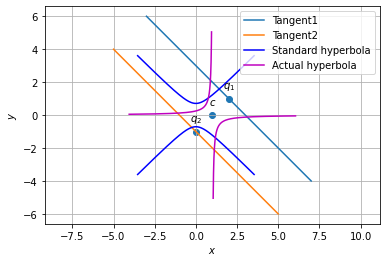
\includegraphics[width=\columnwidth]{./solutions/1/14/graph7.png}
	\caption{The standard and actual hyperbola.}
\end{figure}

\end{enumerate}

\item Two circles intersect at two points $B$ and $C$.
Through $B$, two line segments $ABD$ and $PBQ$
are drawn to intersect the circles at $A, D$ and $P$,
$Q$ respectively. Prove that
$\angle ACP = \angle QCD$.
\item If circles are drawn taking two sides of a triangle as diameters, prove that the point of
intersection of these circles lie on the third side.
\item $ABC$ and $ADC$ are two right triangles with common hypotenuse $AC$. Prove that
$\angle CAD = \angle CBD$.
\item Prove that a cyclic parallelogram is a rectangle.
\item Prove that the line of centres of two intersecting circles subtends equal angles at the
two points of intersection.
\item Let the vertex of an angle $ABC$ be located outside a circle and let the sides of the angle
intersect equal chords $AD$ and $CE$ with the circle. Prove that $\angle ABC$ is equal to half the
difference of the angles subtended by the chords $AC$ and $DE$ at the centre.
\begin{enumerate}
\begin{figure}[!ht]
\centering
\resizebox{\columnwidth}{!}{\renewcommand{\theequation}{\theenumi}
\begin{enumerate}[label=\thesubsection.\arabic*.,ref=\thesubsection.\theenumi]
\numberwithin{equation}{enumi}
	%
%
\item 
%
Draw a circle of radius 3 units.Take two points P and Q on one its extended diameter each at a distance of 7 units from its centre. Draw tangents to the circle from these two points P and Q. 
\\
\solution The given parameters are listed in Table \ref{tab:table1}
%
\begin{table}[!ht]
\begin{center}
\begin{tabular}{ | m{2cm} | m{2cm} |} 
\hline
 & Circle \\
\hline
Centre  & $\vec{O}$=\myvec{0\\0} \\ 
\hline
Radius & $r$=3  \\ 
\hline
Radius & $d$=7  \\ 
\hline
\end{tabular}
\end{center}
\caption{Input values}
\label{tab:table1}
\end{table}
%
\begin{lemma}
  \label{lemma/linman/circ/contact/final}
  The points of contact for the tangent drawn from a point 
%
\begin{align}
  \vec{P} = d\vec{e}_1, \text{ where } \vec{e}_1 = \myvec{1\\0}
  \end{align}
  %
  to the circle are given by 
  \begin{align}
    \vec{x} = \frac{r^2}{d}\vec{e}_1  \pm r\sqrt{1 - \frac{r^2}{d^2}} \vec{e}_2
    \label{linman/circ/contact/final}
   \end{align}
%   
\end{lemma}
If $\vec{x}$ be a point of contact for the tangent from $\vec{P}$, 
\begin{align}
PR &\perp RO
\\
 \implies (\vec{O}-\vec{x})^{\top} (\vec{x}-\vec{P}) &= 0
 \\
 \text{or, }  \vec{P}^{\top} \vec{x} &=\norm{\vec{x}}^2 = r^2
 \\
 \implies \vec{e}_1^{\top} \vec{x} &= \frac{r^2}{d}
  \end{align}
  $\because \vec{O} = 0$.  The above equation can be expressed in parametric form as 
 \begin{align}
  \vec{x} = \frac{r^2}{d}\vec{e}_1 + \lambda \vec{e}_2
  \label{linman/circ/contact}
 \end{align}
 Substituting the above in 
 \begin{align}
  \norm{\vec{x}}^2 = r^2,
 \end{align}
 yields
\begin{align}
\norm{\frac{r^2}{d}\vec{e}_1 + \lambda \vec{e}_2}^2&=r^2
\\
\implies \lambda^2 &= r^2\sbrak{1 - \frac{r^2}{d^2}}
\\
\text{or, }\lambda &= \pm r\sqrt{1 - \frac{r^2}{d^2}}
\end{align}
%
Substituting $\lambda $ in \eqref{linman/circ/contact} yields \eqref{linman/circ/contact/final}.  Fig.  \ref{fig:Tangent lines to circle of radius 3 units.} shows all possible tangents
and their points of contact after substituting the numerical values in \eqref{linman/circ/contact/final}.
%
\begin{figure}[ht]
  \centering
  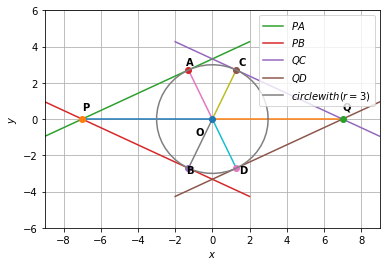
\includegraphics[width=\columnwidth]{solutions/su2021/circle/2/57/FIGURE3.png}
  \caption{Tangent lines to circle of radius 3 units.}
  \label{fig:Tangent lines to circle of radius 3 units.}
\end{figure}
%
\item Draw a  pair of tangents to a circle of radius 5 units  which are inclined to each other at an angle of $60\degree$.
\\
\solution  The angle between the tangents from $\vec{P}$ is given by 
\begin{lemma}
  Given a circle of radius $r$ and angle $\theta$ between the tangents, the intersection of the tangents and points of contact are
  given by Lemma   \ref{lemma/linman/circ/contact/final}  where 
  \begin{align}
    \implies d &= r\sin \frac{\theta}{2}
  \end{align}
%  
\end{lemma}
\begin{proof}
  From Fig.  \ref{fig:Tangent lines to circle of radius 3 units.},
\begin{align}
  \sin \frac{\theta}{2} &= \frac{r}{d}
  \\
  \implies d &= r\sin \frac{\theta}{2}
\end{align}
\end{proof}
Substituting numerical values and plotting, we obtain Fig. \ref{fig:Tangent lines to circle of radius 5 units.}.
%
\begin{figure}[ht]
  \centering
  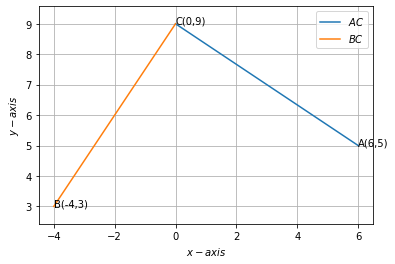
\includegraphics[width=\columnwidth]{solutions/su2021/circle/2/58/download.png}
  \caption{Tangent lines to circle of radius 5 units.}
  \label{fig:Tangent lines to circle of radius 5 units.}
\end{figure}   

\end{enumerate}
}
\caption{}
\label{fig:8.5.49_circle}	
\end{figure}
%
\item {\em Construction: }See Fig. \ref{fig:8.5.49_circle}.  The input parameters are
%
\begin{align}
\label{eq:8.5.49_constr_o}
\vec{O} &= \myvec{0\\0} 
\\
\vec{C} &= \myvec{r\\0} 
\label{eq:8.5.49_constr_c}
\end{align}
Then, 
%
\begin{align}
\label{eq:8.5.49_constr_a}
\vec{A} &= r\myvec{\cos \beta \\ -\sin \beta} 
\end{align}

\subitem Equal chords subtend equal angles at the centre.  Hence 
\begin{align}
\phase{EOC} &= \phase{AOD} = \frac{360 \degree - \alpha -\beta}{2}
\\
&= 180\degree - \frac{\alpha+\beta}{2}
\end{align}
Thus, 
\begin{align}
\vec{D} &= r\myvec{\cos \brak{180^{\circ}-\frac{\alpha+\beta}{2}+\alpha} \\ \sin \brak{180^{\circ}-\frac{\alpha+\beta}{2}+\alpha}} 
\\
 &= r\myvec{-\cos \frac{\alpha-\beta}{2} \\ -\sin \frac{\alpha-\beta}{2}}
\label{eq:8.5.49_constr_d}
\\
\vec{E} &= r\myvec{\cos \brak{180^{\circ}-\frac{\alpha+\beta}{2}} \\ \sin \brak{180^{\circ}-\frac{\alpha+\beta}{2}}}
\\
 &= r\myvec{-\cos \frac{\alpha+\beta}{2} \\ \sin \frac{\alpha+\beta}{2}}
\label{eq:8.5.49_constr_e}
\end{align}
\subitem $\vec{B}$ can be found as the intersection of $AD$ and $CE$.

The given curve 
\begin{align}
	y =\frac{1}{x-1}
\end{align}
can be expressed as 
\begin{align}
	xy - y - 1 = 0 \label{eq:solutions/1/14/eq:hyperbola}
\end{align}
Hence, we have
\begin{align}
	\vec{V} = \frac{1}{2}\myvec{0 & 1 \\ 1 & 0}, 
	\vec{u} = \frac{1}{2}\myvec{0 \\-1},
	f = -1
\end{align}
Since $\mydet{\vec{V}} < 0$, the equation \eqref{eq:solutions/1/14/eq:hyperbola} represents hyperbola.
To find the values of $\lambda_1$ and $\lambda_2$, consider the characteristic equation,
\begin{align}
	\mydet{\lambda\vec{I} - \vec{V}} &= 0\\
	\implies \mydet{\myvec{\lambda & 0\\0 & \lambda} - \myvec{0 & \frac{1}{2} \\ \frac{1}{2} & 0}} &= 0\\
	\implies \mydet{ \lambda & \frac{-1}{2} \\ \frac{-1}{2} & \lambda} &= 0\\
	\implies \lambda_1 &= \frac{1}{2} , \lambda_2 = \frac{-1}{2}
\end{align}
In addition, given the slope -1, the direction and normal vectors are given by 
\begin{align}
	\vec{m} = \myvec{1 \\ -1} \\
	\vec{n} = \myvec{ 1 \\ 1}
\end{align}
The parameters of hyperbola are as follows:
\begin{align}
	\vec{c} &= -\vec{V}^{-1}\vec{u} \\
	&= -\myvec{0 & 2\\ 2 & 0}\myvec{0 \\ -\frac{1}{2}} \\
	&= \myvec{1 \\ 0}\\
	axes &= \begin{cases}
	\sqrt{\frac{\vec{u}^T\vec{V}^{-1}\vec{u} - f}{\lambda_1}} = \sqrt{2}\\
 \sqrt{\frac{f-\vec{u}^T\vec{V}^{-1}\vec{u}}{\lambda_2}} = \sqrt{2}
\end{cases}
\end{align}
which represents the standard hyperbola equation,
\begin{align}
	\frac{x^2}{2} - \frac{x^2}{2} = 1
\end{align}
The points of contact are given by 
\begin{align}
  \tiny{K} &=\pm \sqrt{\frac{\vec{u}^T\vec{V}^{-1}\vec{u} - f}{\vec{n}^T\vec{V}^{-1}\vec{n}}}
  = \pm \frac{1}{2}\\
  \vec{q} &= \vec{V}^{-1}(k\vec{n}-\vec{u})\\
  \vec{q_1} &= \myvec{0 & 2\\2 & 0} \sbrak{\frac{1}{2}\myvec{1 \\ 1} - \myvec{0\\ \frac{-1}{2}}}\\
  &= \myvec{2 \\ 1}\\
  \vec{q_2} &= \myvec{0 & 2\\2 & 0} \sbrak{\frac{-1}{2}\myvec{1 \\ 1} - \myvec{0\\ \frac{-1}{2}}}\\
  &= \myvec{0 \\ -1}
\end{align} 
$\therefore$ The tangents are given by
\begin{align}
	\myvec{1 & 1} \brak{\vec{x} - \myvec{2 \\ 1}} = 0 \\
	\myvec{1 & 1} \brak{\vec{x} - \myvec{0 \\ -1}} = 0
\end{align}
The desired equations of all lines having slope -1 that are tangents to the curve $\frac{1}{x-1}, x \neq 1$ are given by
\begin{align}
	\myvec{1 & 1}\vec{x} &= 3 \\
	\myvec{1 & 1}\vec{x} &= -1 
\end{align}
The above results are verified in the following figure.
\begin{figure}[h!] \label{eq:solutions/1/14/fig:tangents}
	\centering
	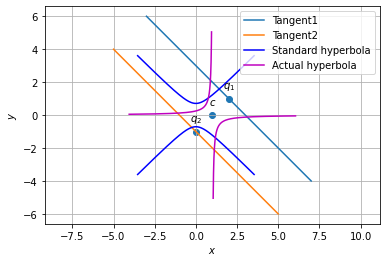
\includegraphics[width=\columnwidth]{./solutions/1/14/graph7.png}
	\caption{The standard and actual hyperbola.}
\end{figure}

\end{enumerate}

\item Prove that the circle drawn with any side of a rhombus as diameter, passes through
the point of intersection of its diagonals.
\item $ABCD$ is a parallelogram. The circle through $A, B$ and $C$ intersect $CD$ (produced if
necessary) at $E$. Prove that $AE = AD$.
\item $AC$ and $BD$ are chords of a circle which bisect each other. Prove that (i) $AC$ and $BD$ are
diameters, (ii) $ABCD$ is a rectangle.
\item Bisectors of angles $A, B$ and $C$ of a $\triangle ABC$ intersect its circumcircle at $D, E$ and
$F$ respectively. Prove that the angles of the $\triangle DEF$ are $90\degree – \frac{A}{2}, 90\degree – \frac{B}{2}$ and $90\degree – \frac{C}{2}$.
\item Two congruent circles intersect each other at points A and B. Through A any line segment PAQ is drawn so that $P, Q$ lie on the two circles. Prove that $BP = BQ$.
\item In any $\triangle ABC$, if the angle bisector of $\angle A$ and perpendicular bisector of $BC$ intersect, prove that they intersect on the circumcircle of the $\triangle ABC$.
%
\item The lengths of tangents drawn from an external point to a circle are equal.
%
\item Prove that in two concentric circles, the chord of the larger circle, which touches the smaller circle, is bisected at the point of contact.
%
\item Two tangents $TP$ and $TQ$ are drawn to a circle with centre $O$ from an external point $T$. Prove that $\angle PTQ = 2 \angle OPQ$.
%
\item Prove that the tangents drawn at the ends of a diameter of a circle are parallel. 
\item  Prove that the perpendicular at the point of contact to the tangent to a circle passes through the centre.
\item A quadrilateral $ABCD$ is drawn to circumscribe a circle. Prove that 
$AB + CD = AD + BC$.
%
\item $XY$ and $X'Y'$ are two parallel tangents to a circle with centre $O$ and another tangent $AB$ with point of contact $C$ intersecting $XY$ at $A$ and $X'Y'$ at $B$. Prove that $\angle AOB = 90\degree$
\item Prove that the angle between the two tangents drawn from an external point to a circle is supplementary to the angle subtended by the line-segment joining the points of contact at the centre.
\item  Prove that the parallelogram circumscribing a circle is a rhombus.
%
\item Prove that opposite sides of a quadrilateral circumscribing a circle subtend supplementary angles at the centre of the circle.
%
\item Find the area of a sector of angle $p$ (in degrees) of a circle with radius $R$. 
\item  Two chords $AB$ and $CD$ intersect each other at the point $P$. Prove that : 
\begin{enumerate}
\item   $\triangle  APC  \sim   \triangle  DPB$
\item  $AP . PB = CP . DP$
\end{enumerate}
\item Two chords $AB$ and $CD$ of a circle intersect each other at the point $P$ (when produced) outside the circle. Prove that 
\begin{enumerate}
\item   $\triangle  PAC  \sim   \triangle  PDB$
\item  $PA . PB = PC . PD$
\end{enumerate}

\end{enumerate}
